\documentclass{standalone}
\usepackage{tikz}
\usepackage{amsfonts,amsmath}

\usepackage{pgfplots}
\usepackage{pgfplotstable}
\usepgflibrary{plotmarks}
\pgfplotsset{compat=newest}

\begin{document}

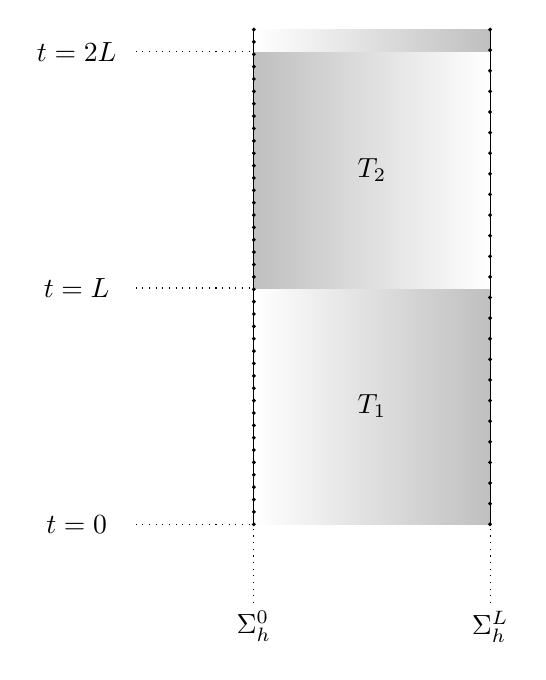
\begin{tikzpicture}
% [every rectangle node/.style={draw},
% every circle node/.style={draw,double}]

\shade[left color=white,right color=lightgray] (0,0) rectangle (3,3) node[pos=.5] {$T_1$};
\shade[left color=lightgray,right color=white] (0,3) rectangle (3,6) node[pos=.5] {$T_2$};
\shade[left color=white,right color=lightgray] (0,6) rectangle (3,2*pi) node[pos=.5] {};

\def\lastx{-0.05}
\draw[black] (0,0)--(0,2*pi);
\draw[black] (3,0)--(3,2*pi);
\foreach \x[remember =\x as \lastx] in {0,2,...,48}{
    \draw (3,\x*pi/24) node[circle, fill =black, scale = 0.1, draw=black] {};
%     \draw (5,\x+5) node[rectangle, fill =orange, scale = 0.4, draw= black,double] {};
%       \draw[ultra thick, lightgray] (5,\lastx+5.05)--(5,5+\x);
%       \draw[ultra thick, lightgray] (0,\lastx+0.05)--(0,0+\x);
    }
\def\lastx{-0.05}
\foreach \x[remember =\x as \lastx] in {0,2,...,80}{
    \draw (0,\x*pi/40) node[circle, fill =black, scale = 0.1, draw= black] {} ;
    % \draw (3,\x) node[circle, fill =blue, scale = 0.4, draw= black, double] {};
%        \draw[ultra thick, black] (0,\lastx+5.05)--(0,5+\x);
%        \draw[ultra thick, black] (5,\lastx+0.05)--(5,0+\x);
    }
\draw[dotted] (-1.5,0)  -- (0,0) node[pos=-0.5] {$t=0$};
\draw[dotted] (-1.5,3)  -- (0,3) node[pos=-0.5] {$t=L$};
\draw[dotted] (-1.5,6)  -- (0,6) node[pos=-0.5] {$t=2L$};
\draw[dotted] (0,-1)  -- (0,0) node[pos=-0.3] {$\Sigma_h^0$};
\draw[dotted] (3,-1)  -- (3,0) node[pos=-0.3] {$\Sigma_h^L$};

\end{tikzpicture}

\end{document}